\documentclass[11pt,a4paper,titlepage]{article}
\usepackage[a4paper]{geometry}
\usepackage[utf8]{inputenc}
\usepackage[english]{babel}
\usepackage{lipsum}

\usepackage{amsmath, amssymb, amsfonts, amsthm, fouriernc, mathtools}
% mathtools for: Aboxed (put box on last equation in align envirenment)
\usepackage{microtype} %improves the spacing between words and letters

\usepackage{graphicx}
\graphicspath{ {./pics/} {./eps/}}
\usepackage{epsfig}
\usepackage{epstopdf}


%%%%%%%%%%%%%%%%%%%%%%%%%%%%%%%%%%%%%%%%%%%%%%%%%%
%% COLOR DEFINITIONS
%%%%%%%%%%%%%%%%%%%%%%%%%%%%%%%%%%%%%%%%%%%%%%%%%%
\usepackage[svgnames]{xcolor} % Enabling mixing colors and color's call by 'svgnames'
%%%%%%%%%%%%%%%%%%%%%%%%%%%%%%%%%%%%%%%%%%%%%%%%%%
\definecolor{MyColor1}{rgb}{0.2,0.4,0.6} %mix personal color
\newcommand{\textb}{\color{Black} \usefont{OT1}{lmss}{m}{n}}
\newcommand{\blue}{\color{MyColor1} \usefont{OT1}{lmss}{m}{n}}
\newcommand{\blueb}{\color{MyColor1} \usefont{OT1}{lmss}{b}{n}}
\newcommand{\red}{\color{LightCoral} \usefont{OT1}{lmss}{m}{n}}
\newcommand{\green}{\color{Turquoise} \usefont{OT1}{lmss}{m}{n}}
%%%%%%%%%%%%%%%%%%%%%%%%%%%%%%%%%%%%%%%%%%%%%%%%%%




%%%%%%%%%%%%%%%%%%%%%%%%%%%%%%%%%%%%%%%%%%%%%%%%%%
%% FONTS AND COLORS
%%%%%%%%%%%%%%%%%%%%%%%%%%%%%%%%%%%%%%%%%%%%%%%%%%
%    SECTIONS
%%%%%%%%%%%%%%%%%%%%%%%%%%%%%%%%%%%%%%%%%%%%%%%%%%
\usepackage{titlesec}
\usepackage{sectsty}
%%%%%%%%%%%%%%%%%%%%%%%%
%set section/subsections HEADINGS font and color
\sectionfont{\color{MyColor1}}  % sets colour of sections
\subsectionfont{\color{MyColor1}}  % sets colour of sections

%set section enumerator to arabic number (see footnotes markings alternatives)
\renewcommand\thesection{\arabic{section}.} %define sections numbering
\renewcommand\thesubsection{\thesection\arabic{subsection}} %subsec.num.

%define new section style
\newcommand{\mysection}{
	\titleformat{\section} [runin] {\usefont{OT1}{lmss}{b}{n}\color{MyColor1}} 
	{\thesection} {3pt} {} } 

%%%%%%%%%%%%%%%%%%%%%%%%%%%%%%%%%%%%%%%%%%%%%%%%%%
%		CAPTIONS
%%%%%%%%%%%%%%%%%%%%%%%%%%%%%%%%%%%%%%%%%%%%%%%%%%
\usepackage{caption}
\usepackage{subcaption}
%%%%%%%%%%%%%%%%%%%%%%%%
\captionsetup[figure]{labelfont={color=Black}}

%%%%%%%%%%%%%%%%%%%%%%%%%%%%%%%%%%%%%%%%%%%%%%%%%%
%		!!!EQUATION (ARRAY) --> USING ALIGN INSTEAD
%%%%%%%%%%%%%%%%%%%%%%%%%%%%%%%%%%%%%%%%%%%%%%%%%%
%using amsmath package to redefine eq. numeration (1.1, 1.2, ...) 
%%%%%%%%%%%%%%%%%%%%%%%%
\renewcommand{\theequation}{\thesection\arabic{equation}}

%set box background to grey in align environment 
\usepackage{etoolbox}% http://ctan.org/pkg/etoolbox
\makeatletter
\patchcmd{\@Aboxed}{\boxed{#1#2}}{\colorbox{black!15}{$#1#2$}}{}{}%
\patchcmd{\@boxed}{\boxed{#1#2}}{\colorbox{black!15}{$#1#2$}}{}{}%
\makeatother
%%%%%%%%%%%%%%%%%%%%%%%%%%%%%%%%%%%%%%%%%%%%%%%%%%

% make the font in the toc 


%\makeatletter
%\let\reftagform@=\tagform@
%\def\tagform@#1{\maketag@@@{(\ignorespaces\textcolor{red}{#1}\unskip\@@italiccorr)}}
%\renewcommand{\eqref}[1]{\textup{\reftagform@{\ref{#1}}}}
%\makeatother
\usepackage{hyperref}
\hypersetup{colorlinks=false}

%%%%%%%%%%%%%%%%%%%%%%%%%%%%%%%%%%%%%%%%%%%%%%%%%%
%% PREPARE TITLE
%%%%%%%%%%%%%%%%%%%%%%%%%%%%%%%%%%%%%%%%%%%%%%%%%%
\title{\blueb Akustische Antenne mit dem Delay \& Sum Algorithmus\\
	\blue Praktikum ADSP \\
	\blue Prof. Dr. Frese}
\author{Jan Kiene}
\date{\today}
%%%%%%%%%%%%%%%%%%%%%%%%%%%%%%%%%%%%%%%%%%%%%%%%%%



\begin{document}
	%{\let\newpage\relax\maketitle}
	
	%\newpage
	{
		\begin{center}
		\blueb
		\LARGE Akustische Antenne mit dem Delay \& Sum - Algorithmus \par
		\centering \large Praktikum ADSP - Jan Kiene	
		\end{center}
	}
	
	\section{Akustische Antenne}
	Eine akustische Antenne ist ein Array aus mehreren Mikrofonen, die in beliebiger Art und Weise angeordnet sein können.
	Die Mikrofone sind dabei so verschaltet, dass sich ein Ausgangssignal für das gesamte Array ergibt.
	Mikrofonarrays können eingesetzt werden, um bestimmte Richtcharakteristika zu erzielen, also den Schall aus einer bestimmten Einfallsrichtung stärker zu gewichten als Schall der aus anderen Richtungen einfällt.
	In der Messtechnik wird diese Eigenschaft genutzt, um Störschallquellen ausfindig zu machen. %(Beispielbild aus Möser??)
	Oft wird auch der Begriff "akustische Kamera" synonym verwendet\footnote{Möser (Hrsg.), Messtechnik der Akustik, Springer 2010, S. 365}.
	\section{Delay \& Sum Algorithmus}

	Der Delay \& Sum Algorithmus ist eine Möglichkeit, eine akustische Antenne zu implementieren. Der Algorithmus beruht auf der Addition ("Sum") der unterschiedlich verzögerten ("Delay") Eingangssignale der einzelnen Mikrofone. Dabei müssen ebene Schallwellen und Kugelschallwellen jeweils unterschiedlich behandelt werden. Generell gilt die Annahme, dass sich Antenne und Quelle im Freifeld befinden (keine Reflexionen).
	
	%Skizze generell
	In Abbildung \ref{fig:das_basic} ist ein beispielhaftes Mikrofonarray dargestellt, bestehend aus $N$ Mikrofonen $m_1,...,m_N$, die im Abstand von $\Delta x$ in einer Reihe angeordnet sind. Eine Schallquelle $Q$ befindet sich im Winkel $\alpha$ vor dem Array.
	Dieser Winkel führt dazu, dass die Schallwelle jedes Mikrofon mit einer bestimmten Verzögerung $\tau_n$ erreicht.
	Die Summe der Mikrofonsignale $p_n(t)$ ist dann
	\begin{equation}
		s_{sum}(t, \alpha) = \sum_{n=1}^{N} p_n(t - \tau_n(\alpha))
	\end{equation}
	Unter der Annahme, dass der Übertragungsweg von der Quelle zur Summierstelle (Luft, Mikrofon, Kabel) keine Signalveränderungen bewirkt, wird also das selbe Signal mit $N-1$ zeitlich verschobenen Kopien von sich selbst addiert.
	Dadurch kommt es zu Auslöschungen und Abschwächungen, sodass generell $RMS(s_{sum}(t, \alpha=0)) \ge RMS(s_{sum}(t, \alpha \ne 0))$.
	
	Die Idee des Delay \& Sum Algorithmus ist nun, die theoretischen Verzögerungszeiten für alle Winkel $\alpha \in [-90^{\circ}, 90^{\circ}]$ zu berechnen und durch nachträgliches "inverses" Verzögern der Mikrofonsignale auszugleichen.
	Anschließend berechnet man von diesen "invers verzögerten" Signalen den Effektivwert und sucht den Winkel, unter dem dieser maximal wurde.
	Dieser Winkel wird dann als Schalleinfallsrichtung angenommen.
	
	\begin{figure}[h]
		\begin{center}
		\includegraphics[scale=0.3]{img/DelaySumDiagram}
		\caption{Beispielhaftes Mikrofonarray mit 8 Mikrofonen mit einer Schalquelle, die eine ebene Welle aus Richtung $\alpha$ emittiert.}
		\label{fig:das_basic}
		\end{center}		
	\end{figure}

\subsection{Delay \& Sum für Ebene Wellen}
	
	Eine Ebene Welle zeichnet sich dadurch aus, dass ihre Wellenfront eine Ebene ist. Die Ausbreitungsrichtung ist also überall gleich.
	Grundsätzlich strahlen "kleine" Quellen (wie zum Beispiel ein Mensch oder ein Lautsprecher) Schall kugelförmig ab. Mit zunehmender Entfernung von der Quelle ähnelt die Schallwelle jedoch immer mehr einer ebenen Welle, sodass ab einer gewissen Distanz von der Schallquelle auch die Annahme einer ebenen Wellenausbreitung getroffen werden kann.
	
	%Skzze ebene Wellen
	Für ebene Wellen stellt sich der Delay \& Sum Algorithmus recht einfach dar. Trifft eine ebene Welle unter dem Winkel $\alpha$ auf das Mikrofonarray, so trifft diese zuerst auf das äußerste Mikrofon und erreicht alle anderen Mikrofone erst nach einer gewissen Verzögerungszeit $\tau_n$.
	Dabei ist speziell für die Annahme ebener Wellen $\tau_n = (n - 1) * \Delta t$. Die Verzögerungszeit zwischen zwei Mikrofonsignalen $\Delta t$ kann mit 
	\begin{equation}
		\Delta t = \frac{\Delta x}{c} = \frac{\Delta x \cdot \sin(\alpha)}{c}
	\end{equation}
	berechnet werden, wobei $c = 340 \frac{m}{s}$ für die Schallgeschwindigkeit in Luft angenommen wird.
	Das Ausgangssignal des Arrays für einen Winkel $\alpha$ berechnet sich dann mit
	\begin{equation}
		s = \sqrt{\frac{1}{T} \int_{0}^{T} \sum_{n=1}^{N} p_m(t - \tau_n(\alpha))}
		\label{eq:das_plane} \footnote{Möser (Hrsg.), Messtechnik der Akustik, Springer 2010, S. 366f}
	\end{equation}
	
	Trägt man den Effektivwert des Arraysignals über dem Winkel auf, so ergibt sich die Richtungsfunktion des Arrays. In Abbildung \ref{fig:bsp_plot} ist beispielhaft die Richtungsfunktion für eine Quelle bei $\alpha = 15^{\circ}$ dargestellt.
	Das Maximum der Effektivwerte ist deutlich bei 15\textdegree\ erkennbar.
	
	\begin{figure}[h]
		\begin{center}
			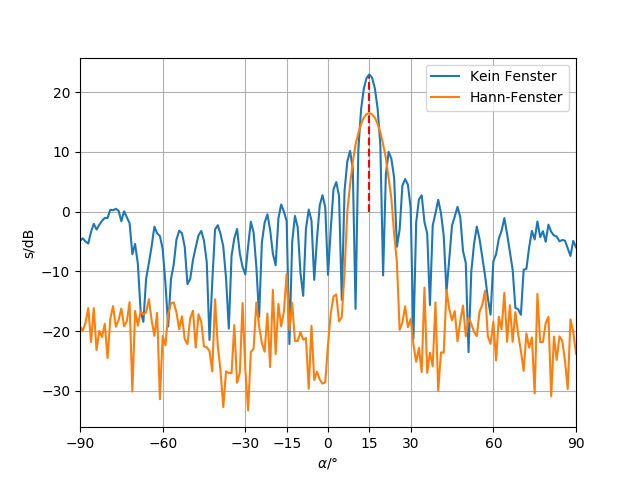
\includegraphics[scale=0.7]{img/bsp_plot_15_beides.png}
			\captionsetup{justification=centering}
			\caption{Richtungsfunktion für eine Quelle bei $\alpha=15^{\circ}$ mit und ohne Gewsichtung. \\
				Das Quellsignal ist ein Sinus mit $f=1000Hz$, das Array hat 20 Mikrofone mit $\Delta x = 0.2m$.\\
				Zum Einsatz kam der Algorithmus für ebene Wellen.}
			\label{fig:bsp_plot}
		\end{center}
	\end{figure}

\subsection{Algorithmus für Kugelwellen}

	\begin{figure}[h]
		\begin{center}
			\includegraphics[scale=0.3]{img/PointSourceDiagram}
			\captionsetup{justification=centering}
			\caption{Situation für Punktschallquellen: Alle möglichen Quellpositionen liegen auf einer Gerade im Abstand $d$ vor dem Mikrofonarray}
		\end{center}
	\end{figure}

	Die meisten realen Schallquellen strahlen Schall kugelförmig ab. Dadurch verkompliziert sich die Berechnung der inversen Delays. Da der Abstand der Quelle zur Arrayachse $d$ für die Berechnung eine Rolle spielt, muss dieser bekannt sein. Der Algorithmus "probiert" dann wieder eine Reihe von Winkeln durch, wobei sich für jeden Winkel ein Punkt $\vec{p}_{\alpha}$ auf einer zur Arrayachse parallelen Geraden im Abstand $d$ mit
	\begin{equation}\vec{p}_{\alpha} = 
		\begin{pmatrix}
			\tan(\alpha) * d \\
			d
		\end{pmatrix}
	\end{equation}
	ergibt. Sollte sich eine Quelle dort befinden, so ist ihre Entfernung zum Mikrofon $m_n$
	\begin{equation}
		r_n = \lvert \vec{p}_{\alpha} - \vec{p}_{n} \rvert
	\end{equation}
	mit
	\begin{equation}
		\vec{p}_n =
		\begin{pmatrix}
			\frac{L}{2} - \Delta x \cdot (n - 1) \\
			0
		\end{pmatrix}
	\end{equation}
	wobei $L$ die Länge des Arrays ist. Die Zeit $\tau_{\alpha, n}$, die eine Schallwelle braucht, um diesen Abstand zurückzulegen kann mit $\tau_{\alpha, n} = \frac{r_n}{c}$ berechnet werden. Werden alle $\tau_{\alpha, n}$ entsprechend ausgeglichen, so ergibt sich für die tatsächliche Quellenposition (beziehungswese für den Winkel, der dieser entspricht) wieder ein Maximum im Effektivwert des Summensignals aller Mikrofone. Es kann so wie für die Annahme ebener Wellen eine Richtungsfunktion bestimmt werden.
	
	Ein wichtiger Unterschied zum Algorithmus für ebene Wellen besteht darin, dass nicht mehr alle Werte in $[-90^{\circ}, 90^{\circ}]$ für $\alpha$ erlaubt sind, da für betraglich größere Winkel das betrachtete Stück der Quellengerade unendlich lang wird. In der vorliegenden Implementierung wird deshalb ein maximaler Betrag für $\alpha$ eingeführt, der einer Quellenposition von 
	\begin{equation}
		\vec{p}_q = 
	\begin{pmatrix}
		\pm L \\
		d
	\end{pmatrix}
	\end{equation}
	entspricht. Damit geht einher, dass der erlaubte Wertebereich von $\alpha$ bei größeren Entfernung zur Quelle kleiner wird.
	

\subsection{Gewichtung der Mikrofone}

	Die Richtungsfunktion lässt sich durch eine Gewichtung der einzelnen Mikrofonsignale verschieden formen. In Abbildung \ref{fig:bsp_plot} ist im Vergleich eine Richtungsfunktion mit und ohne Gewichtung zu sehen.
	Zur Gewichtung der Mikrofone wurde hier die Hann-Fensterfunktion verwendet. Man erkennt, dass das Hauptmaximum deutlich verbreitert wurde, während die Nebenmaxima abgesenkt wurden.
	Allgemein ergibt die Richtungsfunktion mit Gewichtung geringere Werte als ohne.
	Dies resultiert aus der Absenkung der einzelnen Mikrofonsignale durch die Fensterfunktion.
	Je nach Anwendungsfall empfehlen sich verschiedene Fensterfunktionen. Sollen zum Beispiel mehrere Quellen, die eng beieinander liegen, erkannt werden, so wird ein schmaleres Hauptmaximum benötigt\footnote{Möser (Hrsg.), Messtechnik der Akustik, Springer 2010, S. 374ff}.
	\section{Implementierung}
	
	Der Delay \& Sum Algorithmus wurde in der Programmiersprache Python \footnote{Version 3.5.3} implementiert. Benötigt werden neben einer entsprechenden Python-Installation auch noch das Package "numpy" \footnote{Version 1.12.1}. Unter debianbasierten Linuxdistributionen (wie zum Beispiel Ubuntu) kann Python über die Paketquellen und numpy mit "pip" installiert werden, für Windows empfiehlt sich eine Python-Distribution wie zum Beispiel "Anaconda" \footnote{https://www.continuum.io/downloads}.
	
	\subsection{Package delay\_and\_sum}
	
	Das Package enthält die Dateien
	\begin{itemize}
		\item \texttt{delay\_and\_sum.py}
		\item \texttt{signal\_processing.py}
		\item \texttt{\_helper.py}
	\end{itemize}
	In \texttt{delay\_and\_sum.py} wird die Klasse \texttt{DelayAndSumPlane} definiert, die den Delay \& Sum Algorithmus für ebene Wellen umsetzt. Die Methode \texttt{make\_rms\_list} gibt dabei eine Liste mit Effektivwerten für verschiedene Winkel zurück, wie in Gleichung \ref{eq:das_plane} beschrieben.
	Die Klasse \texttt{SignalProcessor} in \texttt{signal\_processing.py} stellt dafür verschiedene Methoden für die Signalverarbeitung zur Verfügung.
	
	Zusäzlich gibt es das \texttt{\_helper.py} Modul, das neben einer Klasse zur Testsignalerzeugung auch Konstanten wie die Schallgeschwindigkeit und Faktoren zur Umrechnung zwischen Bogenmaß und Winkel enthält.
	
\subsection{Bespielskript}

	Das Skript \texttt{locate\_single\_source.py} liest ein Arraysignal aus einer Mehrkanal-Wav-Datei, berechnet den Winkel der aufgenommenen Quelle und zeichnet ein Diagramm mit der Richtungsfunktion.
	Übergeben werden müssen (in dieser Reihenfolge) der Dateiname, die Anzahl der Mikrofone und die Länge des Arrays in Metern. Zusätzlich kann mit dem \texttt{-w} Flag die Gewichtung der Mikrofonsignale mit dem Hann-Fenster angewiesen werden.
	Ein Hilfetext kann mit \texttt{locate\_single\_source.py -h} angezeigt werden.
	
	
\end{document}